\documentclass{clbeamer2024}

\usepackage{minted}

\usepackage{minted}
\setminted{
	breaklines=true,
	frame=single,
	bgcolor=lightgray,
	fontsize=\small,
	escapeinside=||
}

\usepackage{xcolor}
\definecolor{bg}{rgb}{0.95, 0.95, 0.92} % Couleur gris clair

\title{
	%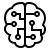
\includegraphics[width=0.5cm]{logos/IA1.png} \hfill
	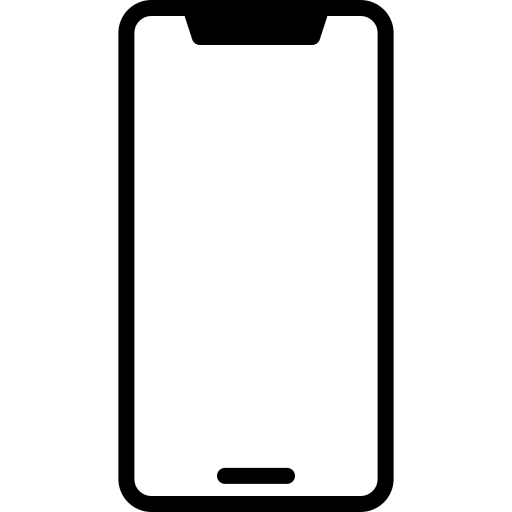
\includegraphics[width=0.7cm]{logos/smartphone.png}
        Introduction à Flutter
	
\includegraphics[width=0.7cm]{logos/flutter.png} \hfill
}
\subtitle{Comprendre les bases du développement multiplateforme}
\author{Slimani Mohamed Amine}
\institute{EHTP}
\date{\today}

\begin{document}
	\setcounter{framenumber}{-1}
	\frame{\titlepage}
	
	
	
	% Sommaire
	\begin{frame}{Sommaire}
		\tableofcontents
	\end{frame}
	
	
	\section{Qu'est-ce que Flutter ?}
	\begin{frame}{Qu'est-ce que Flutter ?}
		\begin{itemize}
			\item \textbf{Définition} : Flutter est un framework de développement d'applications mobiles open-source créé par Google.
			\item \textbf{Objectif} : Permettre de créer des applications natives pour iOS, Android, et le web avec une seule base de code.
			\item \textbf{Avantages} : Performances élevées, développement rapide, interface utilisateur personnalisable.
		\end{itemize}
	\end{frame}
	
	\section{Pourquoi utiliser Flutter ?}
	\begin{frame}{Pourquoi utiliser Flutter ?}
		\begin{itemize}
			\item \textbf{Multiplateforme} : Développez une fois, déployez sur iOS, Android, et le web.
			\item \textbf{Performances} : Moteur de rendu personnalisé pour des animations fluides.
			\item \textbf{Hot Reload} : Visualisez les changements en temps réel sans redémarrer l'application.
		\end{itemize}
	\end{frame}
	
	\section{Composants de Flutter}
	\begin{frame}{Composants de Flutter}
		\begin{itemize}
			\item \textbf{Widgets} : Les éléments de base de l'interface utilisateur (ex : Text, Button, Container).
			\item \textbf{State Management} : Gestion de l'état de l'application (ex : Provider, Riverpod, Bloc).
			\item \textbf{Packages} : Bibliothèques tierces pour étendre les fonctionnalités (ex : http, firebase).
		\end{itemize}
	\end{frame}
	
	
	
	\section{Architecture de Flutter}
	\begin{frame}{Architecture de Flutter}
		\begin{itemize}
			\item \textbf{Widget Tree} : Structure hiérarchique des widgets.
			\item \textbf{State} : Gestion des données et de l'état de l'application.
			\item \textbf{BuildContext} : Contexte de construction des widgets.
		\end{itemize}
		\end{frame}
		
		\section{Exemple de code Flutter}
		
		\begin{frame}{Exemple de code Flutter}
			\begin{exampleblock}{Application Flutter simple}
				
				\begin{figure}[h] % "h" pour placer les images ici
					\centering
					\begin{minipage}{0.6\textwidth}
						\centering
						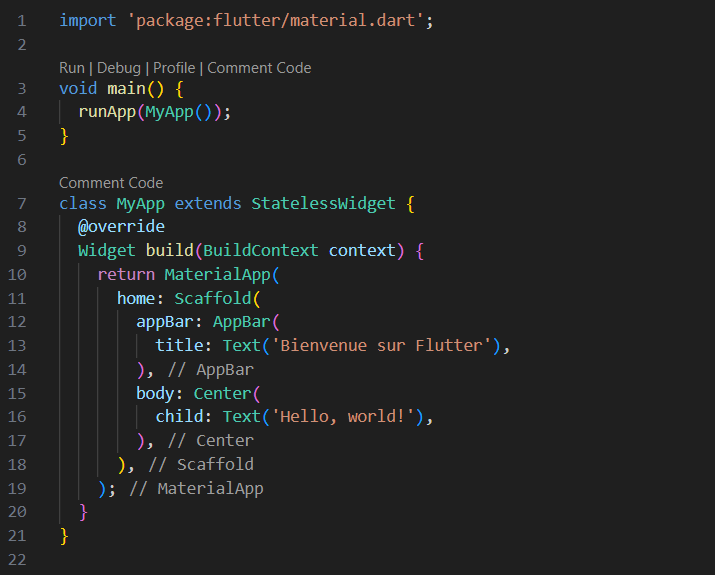
\includegraphics[width=\linewidth]{test/code.png}
						\caption{Code}
						\label{fig:image1}
					\end{minipage}
					\hfill % Espace flexible entre les images
					\begin{minipage}{0.3\textwidth}
						\centering
						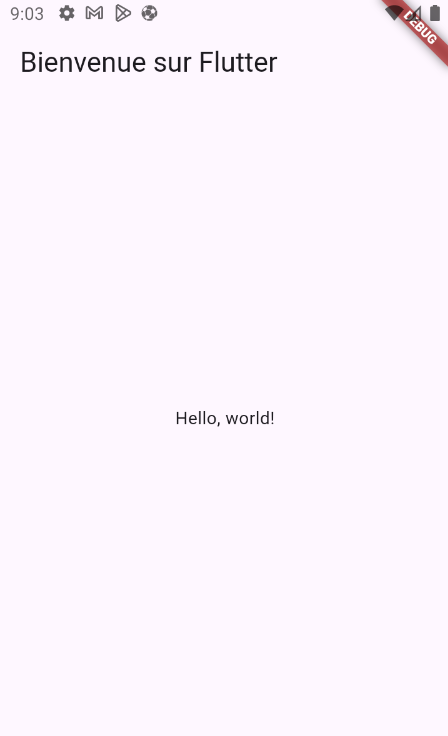
\includegraphics[width=\linewidth]{test/resultat.png}
						\caption{Résultat}
						\label{fig:image2}
					\end{minipage}
				\end{figure}
				
				
			\end{exampleblock}
			
			
		\end{frame}
		
		
		\section{Bonnes pratiques}
		\begin{frame}{Bonnes pratiques}
			\begin{itemize}
				\item \textbf{Utiliser des widgets réutilisables} : Créer des composants modulaires.
				\item \textbf{Gérer l'état efficacement} : Choisir une solution adaptée (Provider, Riverpod, Bloc).
				\item \textbf{Optimiser les performances} : Éviter les reconstructions inutiles de widgets.
			\end{itemize}
		\end{frame}
		
		
		\section{Outils pour travailler avec Flutter}
		\begin{frame}{Outils pour travailler avec Flutter}
			\begin{itemize}
				\item \textbf{Flutter SDK} : Le framework lui-même.
				\item \textbf{Android Studio / VS Code} : Environnements de développement intégrés (IDE).
				\item \textbf{Flutter DevTools} : Outils de débogage et d'analyse des performances.
			\end{itemize}
		\end{frame}

 \section{Défis de Flutter}
 \begin{frame}{Défis de Flutter}
 	\begin{itemize}
 		\item \textbf{Courbe d'apprentissage} : Apprendre Dart et les concepts de Flutter.
 		\item \textbf{Taille de l'application} : Les applications Flutter peuvent être plus volumineuses que les applications natives.
 		\item \textbf{Compatibilité web} : Certaines fonctionnalités ne sont pas encore entièrement supportées sur le web.
 	\end{itemize}
 \end{frame}
 
 \section{Pourquoi c'est important ?}
 \begin{frame}{Pourquoi c'est important ?}
 	\begin{itemize}
 		\item Flutter est un framework puissant pour créer des applications multiplateformes.
 		\item Il offre des performances élevées et un développement rapide.
 		\item Comprendre Flutter est essentiel pour les développeurs mobiles et les concepteurs d'applications.
 	\end{itemize}
 \end{frame}
 
 \begin{frame}{Résumé}
 	\textbf{Flutter} est un framework révolutionnaire pour le développement d'applications multiplateformes.  
 	Développez mieux, plus vite, et avec une seule base de code !  \end{frame}



	
	
\end{document}
